\documentclass[conference]{IEEEtran}

\usepackage{cite}
\usepackage{amsmath,amssymb}
\usepackage{graphicx}
\usepackage{booktabs}
\usepackage{url}

\title{SCIT-Speech: Shared-Codebook Index Transmission for 500--1500 bps Speech Communication}

\author{
\IEEEauthorblockN{Anonymous Authors}
\IEEEauthorblockA{Anonymous Institution\\
Email: anonymous@example.com}
}

\newcommand{\method}{SCIT-Speech}
\newcommand{\base}{SCIT-Speech-Base}
\newcommand{\lca}{SCIT-Speech-LCA}
\newcommand{\codebook}{C^\ast}
\newcommand{\rawrate}{R(L)}

\begin{document}
\maketitle
\begin{abstract}
We introduce \method, a discrete-index speech communication system for 500--1500 bps operation. \method{} treats layered RVQ codebooks and the decoder as pre-shared system knowledge at the transmitter and receiver; at runtime, the channel carries only the first \(L\) RVQ index layers. With \(K=1024\) entries per codebook, a 50 Hz latent frame rate, and three RVQ layers, the ideal index load is \(500L\) bps, yielding 500/1000/1500 bps operating points. Around this interface we make three design choices: a constrained teacher-guided staged NAS protocol that finds a transmitter encoder candidate with 86.9\% fewer parameters, 89.5\% fewer MACs, and 55.1\% lower encoder RTF than the hand-designed SEANet encoder; \base{} training with waveform, multi-scale mel, adversarial, codebook-commitment, and HuBERT semantic distillation losses; and Low-load Channel-aware Adaptation (LCA), which combines random operating-point sampling, strong index-level channel perturbation simulation, and a clean--perturbed mel consistency loss. On LibriSpeech test-clean (\(n=2620\)) and test-other (\(n=2939\)), LCA improves mel-L1 and STOI in all six clean full-set cells, all 12 high-strength index-perturbation cells, and all 12 packet-loss/burst-loss cells. In Whisper base.en ASR evaluation, LCA reduces WER on all test-other clean operating points and all test-other high-perturbation cells, with a maximum reduction of 7.9 percentage points. A single-machine three-client TCP prototype further validates endpoint feasibility: the router forwards index packets only, each client sends one stream and receives two streams, CPU/GPU encode and decode RTF remain below 1, and measured per-end total bandwidth is 11.5--14.5 kbps.
\end{abstract}

\begin{IEEEkeywords}
ultra-low-bitrate speech communication, shared RVQ codebook index transmission, residual vector quantization, channel-aware adaptation, neural audio codec
\end{IEEEkeywords}

\section{Introduction}

Ultra-low-bitrate speech communication remains useful in satellite backhaul, emergency relays, embedded voice front ends, and multi-user edge gateways, where the actual payload available to each speech stream can fall below the operating range of conventional wideband codecs. In the 500--1500 bps regime, the goal is not waveform transparency. A practical system must instead preserve intelligibility, naturalness, and downstream usability under a tightly controlled communication payload.

Recent neural audio codecs and discrete speech representation models such as SoundStream, EnCodec, DAC, SpeechTokenizer, WavTokenizer, and Moshi have shown strong reconstruction quality using residual vector quantization (RVQ) and neural decoders \cite{zeghidour2021soundstream,defossez2022encodec,kumar2023dac,zhang2023speechtokenizer,ji2024wavtokenizer,defossez2024moshi}. However, these systems are usually evaluated at several kbps or above, and their learned codebooks and decoders are treated as model components rather than as an explicit communication interface. Speech semantic communication work, including DeepSC-S, DeepSC-ST, semantic-communication principles, LargeSC, and packet-loss-resilient semantic speech transmission, studies task-aware or semantic transmission, often through continuous joint source-channel mappings or generative recovery modules \cite{weng2021deepscs,weng2022deepscst,qin2022semantic,tian2025largesc,han2025packetloss}. In such systems, the object entering the channel and the corresponding bitrate accounting can depend on modulation, channel symbols, or higher-level protocol assumptions.

This paper studies a narrower question: if the transmitter and receiver pre-share an RVQ codebook family and decoder, can runtime transmission of only the first \(L\) discrete index layers support usable speech communication at 500--1500 bps? We call the resulting shared-codebook index-transmission speech communication system \method. In this interface, bitrate accounting has a closed form, \(L\) becomes a single operating-point knob, and communication errors can be modeled directly on the discrete index sequence as previous-frame coverage, random substitution, packet loss, and burst loss.

The contributions are:
\begin{enumerate}
  \item We formulate shared RVQ codebook index transmission for ultra-low-bitrate speech communication. With \(K=1024\), \(f_q=50\) Hz, and \(n_q=3\), \method{} exposes 500/1000/1500 bps raw/net index-payload operating points.
  \item We give transmitter-side efficiency evidence through a constrained teacher-guided NAS protocol. The selected encoder candidate reduces parameters, MACs, and encoder RTF by 86.9\%, 89.5\%, and 55.1\% relative to the hand-designed SEANet encoder under the same fixed interface. This evidence concerns transmitter efficiency; it is not a claim that the NAS encoder is quality-equivalent after final full training.
  \item We introduce Low-load Channel-aware Adaptation (LCA), composed of random operating-point sampling, channel perturbation simulation, and a mel-domain consistency loss. A V0--V4 factorized ablation quantifies the marginal contribution of these three components.
\end{enumerate}

We evaluate on LibriSpeech test-clean (\(n=2620\)) and test-other (\(n=2939\)) for clean reconstruction and channel perturbations, on Whisper base.en ASR subsets for task-level intelligibility, on VCTK for English cross-corpus zero-shot reconstruction, and in a three-client TCP loopback prototype for endpoint feasibility. We do not claim that \method{} dominates existing codecs at all bitrates or all metrics. Above 6 kbps, Opus and DAC remain stronger choices in many settings. The intended operating range of this paper is 500--1500 bps.

\section{Related Work}

\textbf{Neural audio codecs and discrete speech representations.}
SoundStream, EnCodec, and DAC train end-to-end encoder--quantizer--decoder systems with RVQ bottlenecks for variable-rate neural audio compression \cite{zeghidour2021soundstream,defossez2022encodec,kumar2023dac}. SpeechTokenizer, WavTokenizer, Moshi, and RepCodec explore discrete speech tokens for language modeling, streaming dialogue, or semantic tokenization \cite{zhang2023speechtokenizer,ji2024wavtokenizer,defossez2024moshi,huang2023repcodec}. \method{} keeps the RVQ and layered-token view but repositions the codebooks and decoder as pre-shared system knowledge. The transmitted object is therefore the discrete RVQ index payload rather than a learned latent tensor, waveform, or continuous semantic feature.

\textbf{Semantic feature distillation and semantic-acoustic layering.}
HuBERT hidden-unit prediction has become a common source of frame-level speech representations \cite{hsu2021hubert}. SpeechTokenizer distills semantic information into early RVQ layers; AudioLM and VALL-E use layered discrete representations for audio continuation and zero-shot TTS \cite{zhang2023speechtokenizer,borsos2022audiolm,wang2023valle}. \method{} uses the same broad idea of HuBERT distillation plus multi-layer RVQ, but the objective is different: preserving intelligibility at low \(L\), especially \(L=1\), rather than producing tokens for a downstream language model.

\textbf{Speech semantic communication and packet-loss robustness.}
DeepSC-S, DeepSC-ST, and semantic-communication surveys introduce neural semantic communication systems for speech transmission, recognition, and synthesis \cite{weng2021deepscs,weng2022deepscst,qin2022semantic}. LargeSC and Han et al. further connect semantic communication with large speech models or packet-loss recovery \cite{tian2025largesc,han2025packetloss}. Deep JSCC maps sources directly to channel symbols and motivates end-to-end learned communication under channel noise \cite{bourtsoulatze2018deepjscc}. These systems typically expose continuous semantic vectors or channel symbols as the communication object. In contrast, \method{} keeps a digital discrete interface: the channel carries RVQ indices, the payload has a closed-form accounting rule, and perturbations are modeled on those indices. Neural packet-loss concealment methods synthesize missing waveform segments after decoding \cite{valin2022plc,westhausen2022tplcnet}; LCA instead internalizes robustness into the shared decoder under perturbed index inputs and does not add a second inference network at runtime.

\textbf{Neural architecture search for efficient speech models.}
DARTS and ProxylessNAS established differentiable and hardware-aware NAS principles \cite{liu2018darts,cai2018proxylessnas}. LightSpeech applied NAS to lightweight TTS models \cite{luo2021lightspeech}. Our NAS protocol is narrower: it searches only the transmitter-side encoder under a fixed low-bitrate speech communication interface, with fixed latent dimensionality, downsampling, frame rate, RVQ depth, and codebook size. The searched encoder is used as transmitter-side efficiency evidence, while final reconstruction claims are based on the full \base{} and \lca{} training and evaluation.

\section{Method}

\begin{figure*}[t]
  \centering
  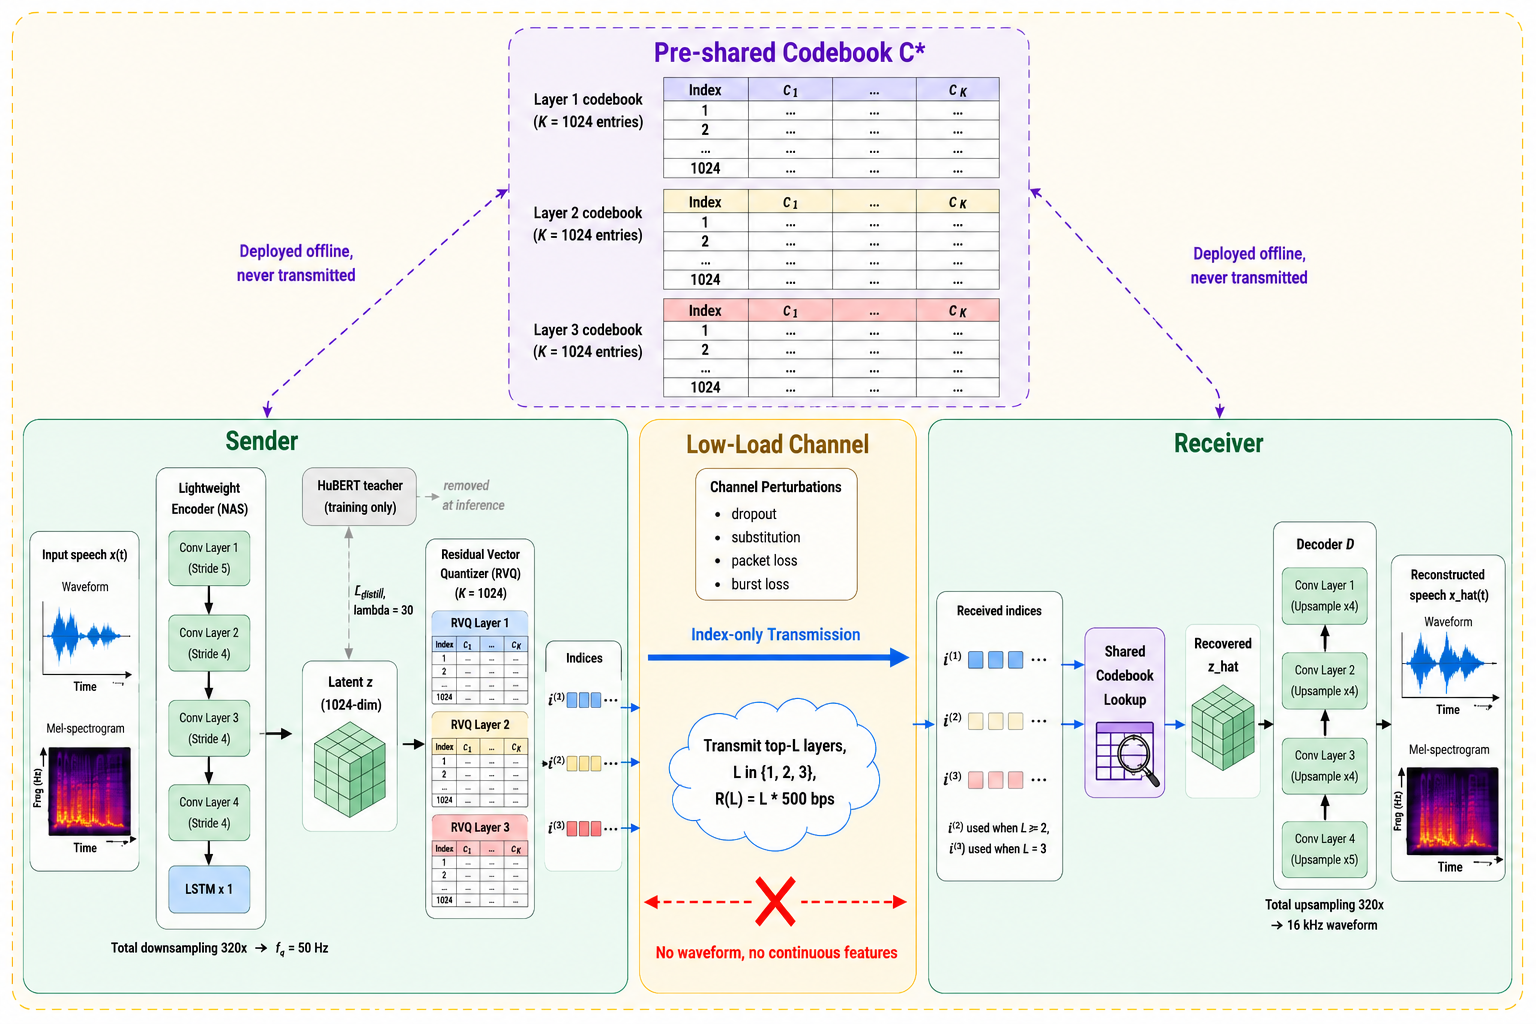
\includegraphics[width=0.95\textwidth]{figures/图片1.png}
  \caption{\method{} system overview. The transmitter and receiver pre-share the RVQ codebooks \(\codebook\), decoder \(D\), and configuration. Runtime packets contain only the first \(L\) layers of RVQ indices. LCA trains the shared decoder to reconstruct robustly from truncated and perturbed index sequences; the HuBERT teacher is used only during Base training.}
  \label{fig:overview}
\end{figure*}

Figure~\ref{fig:overview} summarizes \method. The input waveform is encoded, quantized by a multi-layer RVQ, truncated to the first \(L\) index layers, optionally perturbed by the channel, and decoded by the receiver using pre-shared codebooks and decoder parameters.

\textbf{Notation.}
We use \(x\) for the input waveform, \(\hat{x}\) for the reconstruction, \(E_\theta\) for the encoder, \(D\) for the pre-shared decoder, \(\codebook\) for the pre-shared RVQ codebook family, \(Z\) for the continuous encoder output before quantization, \(q^{(1)}\) for the first-layer quantized feature used in semantic distillation, \(I\) for the full RVQ index tensor, \(I_{1:L}\) for its first \(L\) layers, and \(\tilde{I}_{1:L}\) for the channel-perturbed indices.

\subsection{Shared RVQ Codebook Index Transmission}

Let \(x\) be an input waveform, \(E_\theta\) the encoder, \(Z=E_\theta(x)\in\mathbb{R}^{T_q\times d}\) the continuous latent sequence, \(M=n_q\) the number of RVQ layers, and \(I=\{i_{m,t}\}\) the full index tensor. The transmitter and receiver pre-share the RVQ codebook family \(\codebook=\{C_1^\ast,\ldots,C_M^\ast\}\), decoder \(D\), and system configuration. At runtime, the transmitter sends only
\[
I_{1:L}=\{i_{m,t}:1\leq m\leq L,\;1\leq t\leq T_q\},
\]
and the receiver reconstructs
\[
\hat{x}=D(\codebook(I_{1:L})).
\]

The current system uses \(M=n_q=3\), \(K=1024\), 16 kHz audio, total downsampling 320, and latent frame rate \(f_q=50\) Hz. With fixed 10-bit packing per index,
\[
\rawrate = L f_q \lceil \log_2 K\rceil = 500L\;\text{bps}, \qquad L\in\{1,2,3\}.
\]
Thus \(L=1,2,3\) correspond to raw/net index payloads of 500, 1000, and 1500 bps, or approximately \(512\times\), \(256\times\), and \(171\times\) compression relative to 16 kHz, 16-bit PCM. The fixed-packing payload is a conservative midpoint between entropy-coded payload and packetized online bandwidth. Empirical index histograms over 600 evaluation utterances give entropy lower bounds of roughly 398--415 bps for \(L=1\), 838--882 bps for \(L=2\), and 1301--1356 bps for \(L=3\). Real online bitrate is higher because of packetization and protocol headers: for example, RTP-only 100 ms packetization adds about 204\%, 100\%, and 65\% over \(500L\) at \(L=1,2,3\), while UDP/IPv4/RTP adds about 652\%, 334\%, and 215\%. The experiments report \(500L\) bps for codec comparison and separately report prototype body and total bandwidth in Section~\ref{sec:prototype}.

\subsection{Constrained NAS Transmitter Encoder}

The transmitter encoder is searched under a fixed interface contract: latent dimension 1024, total downsampling 320, latent frame rate 50 Hz, \(K=1024\), \(n_q=3\), and a decoder stride sequence derived from the encoder stride sequence. The search space varies six stride patterns, three channel widths, two residual-compression ratios, one or two LSTM layers, ELU/Snake activation, per-block convolutional operators, optional squeeze-excitation, and at most one skipped encoder block.

The four-stage protocol is teacher-guided. Stage 1 samples 8192 candidates and applies resource gating using a weighted log-ratio score over MACs, parameters, and encoder RTF relative to a hand-designed SEANet encoder, retaining 512 candidates. Stage 2 performs 100-step short distillation against a frozen teacher latent representation and ranks candidates using resource terms plus one-sided quality penalties, retaining 64 candidates. Stage 3 extends distillation to 500 steps, checks RVQ-compatibility diagnostics on a 16-sample subset, and retains 8 candidates. Stage 4 extends distillation to 1500 steps and chooses from a Pareto frontier over seven quality/proxy objectives and three resource objectives. These proxy losses rank candidates only; final quality claims use the fully trained \base{} and \lca{} checkpoints.

The selected encoder uses strides \([5,4,4,4]\), 24 filters, compression 2, one LSTM layer, Snake activation, and four blocks consisting of skip, standard convolution with kernel 7, separable convolution with kernel 9, and dilated convolution with kernel 5. Under the same efficiency measurement protocol, it has 8.87M parameters, 0.618G MAC/s, and encoder RTF 0.00368, compared with 67.7M parameters, 5.87G MAC/s, and RTF 0.00819 for the hand-designed SEANet encoder. These measurements support transmitter-side efficiency only; final speech quality is evaluated after the full Base and LCA training procedures below.

\subsection{\base{} Training}

\base{} follows the neural codec training pattern of an RVQ generator with adversarial discriminators. The generator includes \(E_\theta\), the RVQ quantizer, and decoder \(D\), and is trained on LibriSpeech train-clean-100. The key layering choice is to apply HuBERT semantic distillation to the first RVQ-layer quantized feature \(q^{(1)}\), encouraging layer 1 to carry frame-level semantic information while later RVQ layers add acoustic residual detail. The generator objective is
\[
\begin{split}
\mathcal{L}_{\mathrm{full}} &=
\mathcal{L}_{\mathrm{mel}}(x,\hat{x})
 + \lambda_{\mathrm{recon}}\mathcal{L}_{\mathrm{recon}}(x,\hat{x}) \\
&\quad + \mathcal{L}_{\mathrm{adv}} + \mathcal{L}_{\mathrm{feat}}
 + \lambda_q \mathcal{L}_{\mathrm{commit}} \\
&\quad + \lambda_{\mathrm{distill}}
 \mathcal{L}_{\mathrm{distill}}(q^{(1)},h^{\mathrm{H}}(x)).
\end{split}
\]
Here \(\mathcal{L}_{\mathrm{recon}}=\|x-\hat{x}\|_1\), \(\mathcal{L}_{\mathrm{mel}}\) is a four-scale log-mel loss, \(\mathcal{L}_{\mathrm{adv}}\) and \(\mathcal{L}_{\mathrm{feat}}\) are adversarial and feature-matching losses, and \(\mathcal{L}_{\mathrm{commit}}\) is the RVQ commitment loss. The HuBERT term aligns \(q^{(1)}\), not the full encoder output, to HuBERT teacher features using a cosine-similarity logistic objective. The teacher branch is removed at inference time.

\subsection{Low-load Channel-aware Adaptation}

LCA fine-tunes \base{} with a full-depth branch and a communication branch:
\[
\mathcal{L}_{\mathrm{LCA}} = \lambda_{\mathrm{full}}\mathcal{L}_{\mathrm{full}}
 + \lambda_{\mathrm{comm}}\mathcal{L}_{\mathrm{comm}}.
\]
The communication branch has three components.

\textbf{Random operating-point sampling.}
At each training step, LCA samples \(L\in\{1,2,3\}\) uniformly and truncates the full RVQ index tensor to \(I_{1:L}\). Step-level sampling keeps all samples in the same forward pass at the same operating point.

\textbf{Channel perturbation simulation.}
Each step samples one of five channel conditions: clean, medium previous-frame coverage (\(p_{\mathrm{drop}}=0.05\)), high previous-frame coverage (\(p_{\mathrm{drop}}=0.10\)), medium random substitution (\(p_{\mathrm{sub}}=0.01\)), or high random substitution (\(p_{\mathrm{sub}}=0.03\)). Previous-frame coverage independently selects index positions and replaces them by the original \(t-1\) index in the same layer; \(t=0\) is not modified, and consecutive hits do not iteratively propagate filled values. Random substitution replaces selected positions by uniformly sampled codebook indices. The two perturbation types are mutually exclusive at the condition level. Packet loss and burst loss are not used during training; they are evaluation-only distribution shifts.

\textbf{Mel-domain consistency.}
Let \(\tilde{I}_{1:L}\) denote the perturbed index sequence. The decoder produces
\[
\hat{x}_{\mathrm{clean}}=D(\codebook(I_{1:L})),\qquad
\hat{x}_{\mathrm{pert}}=D(\codebook(\tilde{I}_{1:L})).
\]
The communication reconstruction term applies the same mel and waveform losses to \(\hat{x}_{\mathrm{pert}}\). When the sampled condition is perturbed, LCA also adds
\[
\mathcal{L}_{\mathrm{consistency}} =
\sum_s w_s \|\phi_s(\hat{x}_{\mathrm{clean}})-\phi_s(\hat{x}_{\mathrm{pert}})\|_1,
\]
where \(\phi_s\) are the same multi-scale log-mel operators as in Base training. The final communication loss is
\[
\begin{aligned}
\mathcal{L}_{\mathrm{comm}} &=
\mathcal{L}_{\mathrm{comm\_recon}} \\
&\quad + \lambda_{\mathrm{consistency}}\mathbf{1}_{\mathrm{pert}}
\mathcal{L}_{\mathrm{consistency}} .
\end{aligned}
\]
We use \(\lambda_{\mathrm{full}}=1.0\), \(\lambda_{\mathrm{comm}}=1.5\), and \(\lambda_{\mathrm{consistency}}=0.5\). Gradients from the communication branch flow through the decoder only; the truncated and perturbed indices are treated as stop-gradient inputs. This design trains the shared decoder to recover from low-\(L\) and perturbed indices without directly training the encoder or quantizer through the channel simulator.

\section{Experimental Setup}

\textbf{Data.}
Models are trained on LibriSpeech train-clean-100. Main evaluation uses LibriSpeech test-clean (\(n=2620\)) and test-other (\(n=2939\)). Same-bitrate codec comparison uses the first 300 samples from each split, denoted test-clean-300 and test-other-300. Perturbed ASR uses the first 100 samples from those 300-sample subsets. Cross-corpus zero-shot evaluation uses 300 VCTK utterances sampled uniformly across speakers with seed 42, without retraining or fine-tuning. None of these evaluation subsets is used for model selection.

\textbf{Models and baselines.}
The \method{} family includes \base{} trained for 60 epochs and \lca{} v2 fine-tuned for 10 epochs from Base. Same-bitrate and reference baselines are PCM, Opus at 6/8/12/16/24 kbps, EnCodec 24 kHz at 1.5/3.0/6.0/12.0 kbps, DAC 16 kHz with \(n_q\in\{1,2,3,4,6,9,12\}\), AMR-WB at 6.6--23.85 kbps, and Codec2 at 700C/1200/1300/1600/2400/3200 bps \cite{valin2012opus,defossez2022encodec,kumar2023dac,itu2002amrwb,codec2repo}. AMR-WB and Codec2 are evaluated with an ffmpeg build containing the required encoders; all baselines use public weights or public codec implementations without task-specific fine-tuning.

\textbf{Perturbations.}
Index-level perturbations reuse the LCA ChannelSim conditions from Section~3.4. Communication-style perturbations are evaluation-only: packet loss drops 100 ms packets with 1\%, 3\%, or 5\% probability, and burst loss drops contiguous spans of 2, 5, or 10 latent frames. In lost packet or burst spans, the receiver fills with the last index before the missing span.

\textbf{Metrics.}
We report mel-L1, STOI \cite{taal2011stoi}, PESQ-WB \cite{itu2001pesq}, SI-SNR, ViSQOL v3 speech-mode MOS-LQO \cite{chinen2020visqol}, and Whisper base.en WER/CER \cite{radford2022whisper}. Whisper uses deterministic greedy decoding with `condition\_on\_previous\_text=False' and a shared text-normalization chain before WER/CER computation. PCM passthrough gives a corpus WER floor of 0.0359 on test-clean-300 and 0.1552 on test-other-300. Paired comparisons use matched samples, operating points, and channel seeds.

\textbf{Training details.}
Training uses 1 s waveform segments at 16 kHz, batch size 8, gradient accumulation 4, Adam with \(\beta_1=0.9\), \(\beta_2=0.99\), no weight decay, cosine annealing, bf16 mixed precision, and seed 42. The loss weights are \(\lambda_{\mathrm{recon}}=500\), \(\lambda_q=10\), and \(\lambda_{\mathrm{distill}}=30\). The four log-mel scales use \((n_{\mathrm{fft}},\mathrm{hop},\mathrm{win})\) values
\[
\begin{gathered}
(1024,240,1024),\ (512,120,512),\\
(256,60,256),\ (128,30,128),
\end{gathered}
\]
with weights \([45,1,1,1]\). \base{} is trained from scratch with learning rate \(10^{-4}\) and selected by validation mel-L1. \lca{} loads the \base{} generator, restarts the discriminator, optimizer, and scheduler, fine-tunes with learning rate \(10^{-5}\), and validates every 2500 steps over a \(3L\times5\)-condition communication mel matrix. The official LCA checkpoint is selected at step 30000, where high random substitution at \(L=1,2,3\) jointly reaches the best dev communication mel error.

\section{Results}

\subsection{Same-bitrate Comparison}

\begin{figure*}[t]
  \centering
  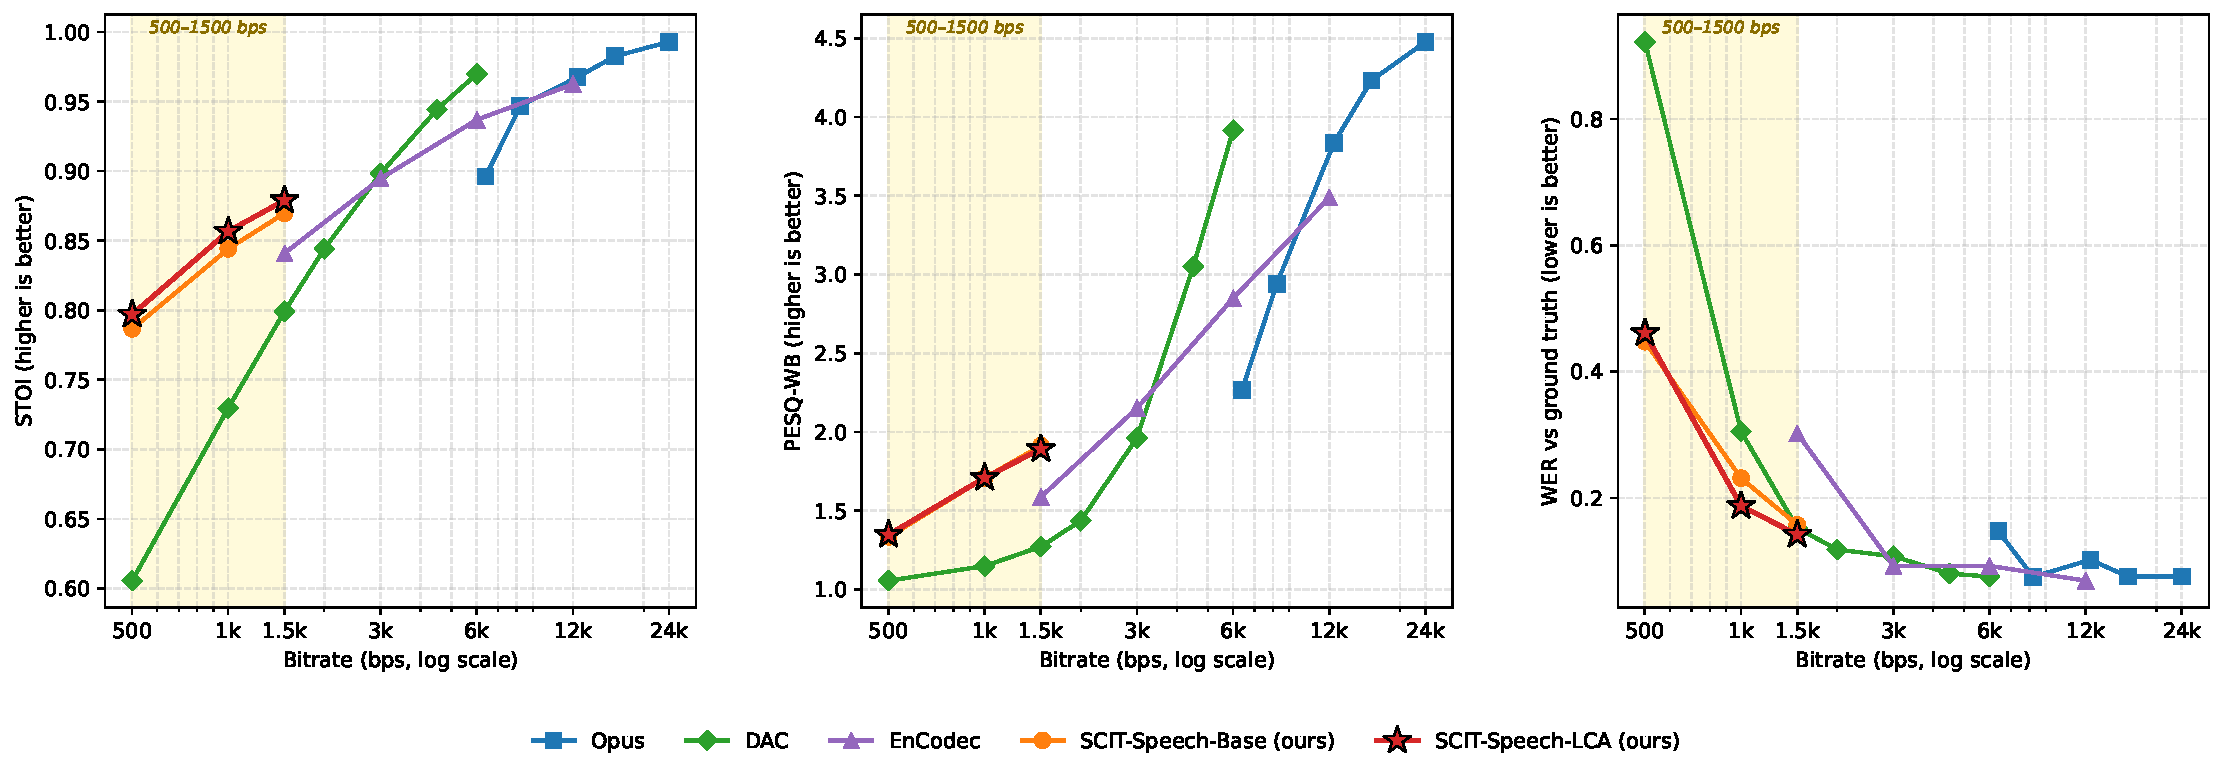
\includegraphics[width=0.95\textwidth]{figures/fig2_rate_quality_tradeoff.pdf}
  \caption{Rate-quality trade-off on test-clean-300 and test-other-300. The three panels show mel-L1, STOI, and PESQ-WB against actual packed bitrate on a log scale. The shaded band marks the 500--1500 bps \method{} operating range; error bars denote 95\% bootstrap confidence intervals.}
  \label{fig:rate_quality}
\end{figure*}

Figure~\ref{fig:rate_quality} and Table~\ref{tab:same_bitrate} summarize the same-bitrate comparison. At 500/1000/1500 bps, \lca{} is consistently better than same-rate DAC in mel-L1, STOI, and PESQ-WB on both LibriSpeech subsets. At 1500 bps, \lca{} is also better than EnCodec 1.5 kbps on these three metrics. All corresponding paired Wilcoxon tests in the Chinese source draft have \(p<0.001\). The main exception inside the \method{} family is test-other at \(L=1\), where LCA has slightly worse mel-L1 than Base but better STOI and PESQ-WB.

\begin{table*}[t]
\centering
\caption{Key same-bitrate results on LibriSpeech 300-sample subsets. Values are mean with 95\% bootstrap confidence intervals from the source draft. ViSQOL is MOS-LQO.}
\label{tab:same_bitrate}
\small
\resizebox{\linewidth}{!}{%
\begin{tabular}{llccccc}
\toprule
Subset & Method & Bitrate & mel-L1 \(\downarrow\) & STOI \(\uparrow\) & PESQ-WB \(\uparrow\) & ViSQOL \(\uparrow\) \\
\midrule
test-clean & \lca{} \(L=1\) & 500 bps & \textbf{1.122 [1.108, 1.137]} & \textbf{0.822 [0.819, 0.826]} & 1.390 [1.379, 1.402] & 1.540 [1.502, 1.579] \\
test-clean & DAC \(n_q=1\) & 501 bps & 2.049 [2.027, 2.071] & 0.623 [0.618, 0.628] & 1.064 [1.060, 1.069] & 1.214 [1.196, 1.231] \\
test-clean & Codec2 700C & \(\sim\)815 bps & 3.730 [3.683, 3.781] & 0.532 [0.526, 0.538] & \textbf{1.408 [1.388, 1.430]} & \textbf{1.613 [1.577, 1.651]} \\
test-clean & \lca{} \(L=2\) & 1000 bps & \textbf{0.898 [0.887, 0.911]} & \textbf{0.879 [0.876, 0.882]} & \textbf{1.823 [1.800, 1.847]} & 2.094 [2.042, 2.146] \\
test-clean & DAC \(n_q=2\) & 1002 bps & 1.453 [1.440, 1.465] & 0.740 [0.736, 0.744] & 1.150 [1.141, 1.159] & 1.354 [1.328, 1.381] \\
test-clean & Codec2 1200 & \(\sim\)1.2 kbps & 3.245 [3.214, 3.276] & 0.667 [0.662, 0.671] & 1.621 [1.589, 1.654] & \textbf{2.128 [2.083, 2.173]} \\
test-clean & \lca{} \(L=3\) & 1500 bps & \textbf{0.838 [0.825, 0.851]} & \textbf{0.900 [0.897, 0.903]} & \textbf{2.097 [2.066, 2.128]} & \textbf{2.393 [2.340, 2.445]} \\
test-clean & EnCodec 1.5k & 1502 bps & 1.282 [1.266, 1.297] & 0.848 [0.845, 0.851] & 1.612 [1.585, 1.638] & 2.028 [1.978, 2.079] \\
test-clean & Codec2 1300 & \(\sim\)1.4 kbps & 3.644 [3.609, 3.680] & 0.661 [0.656, 0.665] & 1.428 [1.402, 1.456] & 1.917 [1.878, 1.956] \\
\midrule
test-other & \lca{} \(L=1\) & 500 bps & 1.543 [1.502, 1.586] & \textbf{0.793 [0.788, 0.797]} & \textbf{1.312 [1.296, 1.329]} & \textbf{1.656 [1.609, 1.703]} \\
test-other & DAC \(n_q=1\) & 501 bps & 2.326 [2.292, 2.360] & 0.603 [0.598, 0.608] & 1.045 [1.042, 1.047] & 1.294 [1.269, 1.320] \\
test-other & Codec2 700C & \(\sim\)815 bps & 4.075 [4.023, 4.127] & 0.489 [0.483, 0.494] & 1.279 [1.262, 1.297] & 1.508 [1.470, 1.546] \\
test-other & \lca{} \(L=2\) & 1000 bps & \textbf{1.269 [1.219, 1.322]} & \textbf{0.838 [0.834, 0.843]} & \textbf{1.588 [1.555, 1.622]} & 1.785 [1.723, 1.846] \\
test-other & DAC \(n_q=2\) & 1002 bps & 1.696 [1.666, 1.726] & 0.726 [0.722, 0.729] & 1.102 [1.093, 1.111] & 1.641 [1.604, 1.678] \\
test-other & Codec2 1200 & \(\sim\)1.2 kbps & 3.445 [3.417, 3.472] & 0.647 [0.642, 0.651] & 1.370 [1.347, 1.394] & \textbf{2.013 [1.956, 2.070]} \\
test-other & \lca{} \(L=3\) & 1500 bps & \textbf{1.190 [1.139, 1.244]} & \textbf{0.857 [0.853, 0.862]} & \textbf{1.756 [1.715, 1.797]} & \textbf{1.956 [1.885, 2.027]} \\
test-other & EnCodec 1.5k & 1502 bps & 1.666 [1.624, 1.708] & 0.826 [0.822, 0.829] & 1.521 [1.498, 1.544] & 1.772 [1.719, 1.825] \\
test-other & Codec2 1300 & \(\sim\)1.4 kbps & 3.634 [3.602, 3.666] & 0.652 [0.647, 0.656] & 1.310 [1.289, 1.330] & 1.633 [1.592, 1.672] \\
\bottomrule
\end{tabular}
}
\end{table*}

Across the three target operating points, \lca{} significantly outperforms same-rate DAC in mel-L1, STOI, and PESQ-WB on both subsets. At 1500 bps, \lca{} also improves over EnCodec 1.5 kbps on these metrics. All corresponding paired Wilcoxon tests in the source draft have \(p<0.001\). The main exception inside the \method{} family is test-other \(L=1\), where LCA has slightly higher mel-L1 than Base but still improves STOI/PESQ-WB and remains better than DAC. Codec2 is the only traditional baseline in the 500--1500 bps neighborhood: under mel-L1, STOI, and PESQ-WB it is generally worse than \lca{}, but ViSQOL gives a more conservative view and keeps Codec2 competitive at a few low-rate points.

\subsection{ViSQOL Perceptual Quality}

\begin{figure}[t]
  \centering
  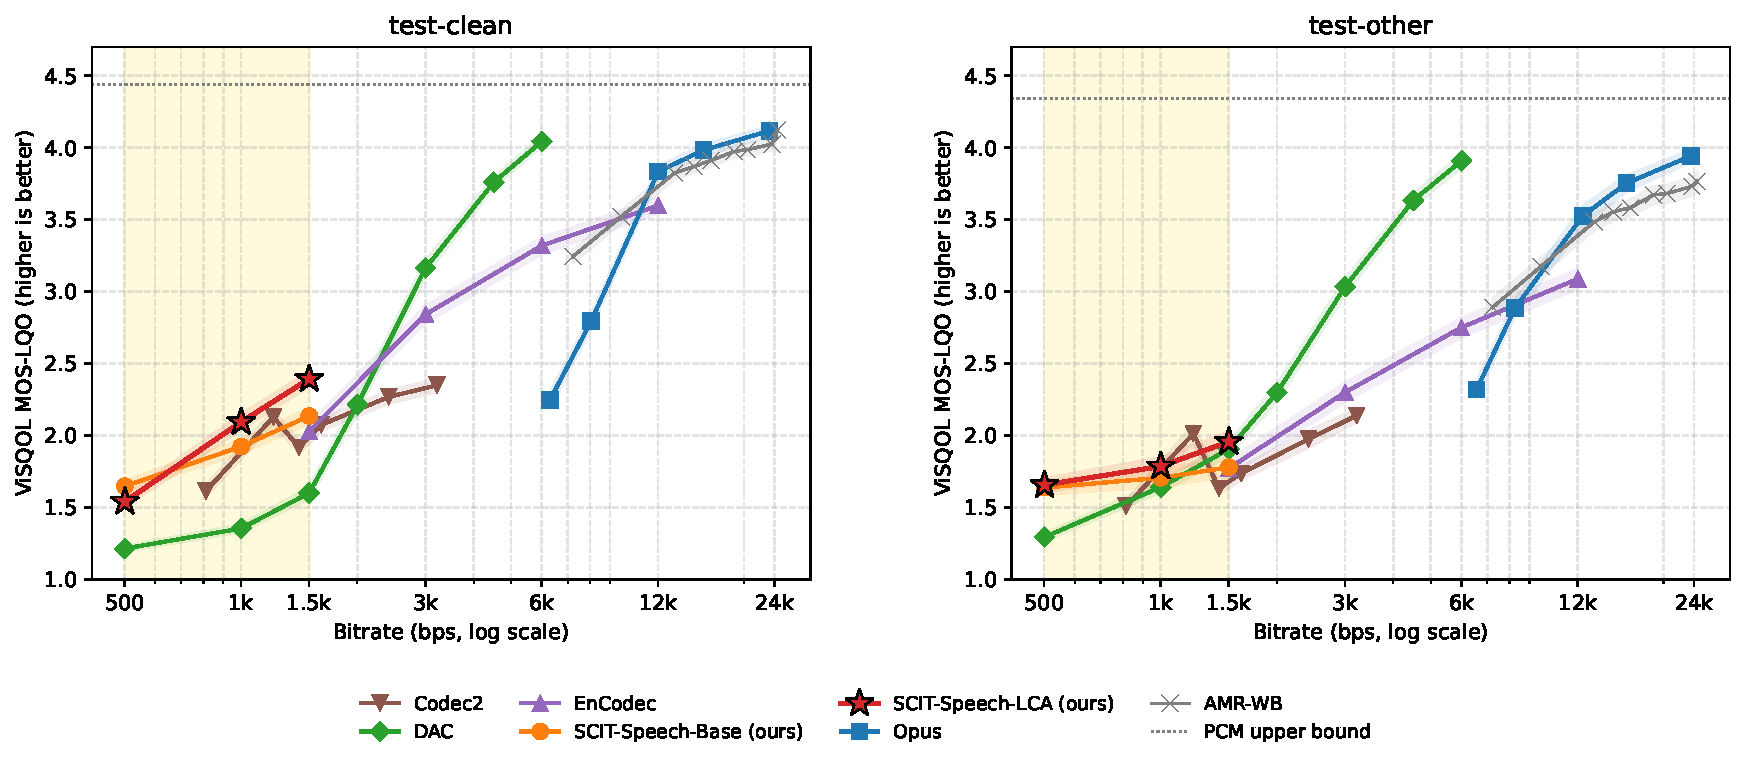
\includegraphics[width=\linewidth]{figures/fig3_visqol.pdf}
  \caption{ViSQOL MOS-LQO against bitrate on test-clean-300 and test-other-300. The dotted line is the PCM upper bound under this metric; the shaded band marks 500--1500 bps.}
  \label{fig:visqol}
\end{figure}

Figure~\ref{fig:visqol} and Table~\ref{tab:visqol} show that \lca{} remains better than same-rate neural codecs under ViSQOL. The comparison with Codec2 is mixed: \lca{} is worse at test-clean \(L=1\) and test-other \(L=2\), statistically tied at test-clean \(L=2\), and better at the remaining displayed Codec2 points. This is why the claim is stated as consistent superiority over same-rate neural codecs, not dominance over every specialized low-rate speech codec under every metric. PCM passthrough gives an experiment-specific ViSQOL upper bound of about 4.44 on test-clean and 4.34 on test-other; ViSQOL does not return the theoretical maximum 5.0 even for identical references in this setup.

\begin{table}[t]
\centering
\caption{ViSQOL differences \(\Delta\)MOS-LQO = \lca{} minus baseline.}
\label{tab:visqol}
\small
\begin{tabular}{lccc}
\toprule
Point & vs DAC & vs Codec2 & vs EnCodec \\
\midrule
500 bps clean & +0.33 & -0.07 & -- \\
500 bps other & +0.36 & +0.15 & -- \\
1000 bps clean & +0.74 & -0.03 & -- \\
1000 bps other & +0.15 & -0.23 & -- \\
1500 bps clean & +0.79 & +0.48 & +0.37 \\
1500 bps other & +0.05 & +0.32 & +0.19 \\
\bottomrule
\end{tabular}
\end{table}

\subsection{Clean Full-set Generalization}

Before interpreting perturbation robustness, we test whether LCA sacrifices clean reconstruction. Table~\ref{tab:clean_full} shows the full LibriSpeech clean evaluation. LCA improves mel-L1 and STOI in all six cells. PESQ-WB improves only at \(L=1\) and slightly decreases at \(L=2,3\); SI-SNR is also mixed. Thus, LCA does not obtain robustness by broadly degrading clean spectral quality, but the gains are concentrated in mel/STOI rather than waveform alignment.

\begin{table}[t]
\centering
\caption{Full-set clean evaluation. \(\Delta\) denotes LCA minus Base.}
\label{tab:clean_full}
\small
\begin{tabular}{llrrrr}
\toprule
Subset & \(L\) & \(\Delta\)mel & \(\Delta\)STOI & \(\Delta\)PESQ & \(\Delta\)SI-SNR \\
\midrule
clean & 1 & -0.021 & +0.013 & +0.023 & -0.36 \\
clean & 2 & -0.030 & +0.007 & -0.019 & -0.29 \\
clean & 3 & -0.036 & +0.007 & -0.014 & +0.01 \\
other & 1 & -0.013 & +0.013 & +0.024 & -0.31 \\
other & 2 & -0.030 & +0.008 & -0.010 & -0.36 \\
other & 3 & -0.033 & +0.007 & -0.015 & -0.03 \\
\bottomrule
\end{tabular}
\end{table}

\subsection{Index Perturbation, Packet Loss, and Burst Loss}

Under high previous-frame coverage and high random substitution, LCA improves mel-L1 and STOI in all 12 full-set evaluation cells, with mel-L1 changes from \(-0.018\) to \(-0.048\) and STOI changes from \(+0.008\) to \(+0.017\). Under evaluation-only packet loss and burst loss, LCA again improves mel-L1 and STOI in all 12 cells. PESQ-WB is mostly improved for index-level perturbations but mixed for packet and burst losses. SI-SNR is mixed, which is consistent with the source draft's interpretation that LCA stabilizes spectral and intelligibility-related behavior more than exact waveform alignment.

\begin{table*}[t]
\centering
\caption{Full-set high index perturbation and evaluation-only loss robustness. \(\Delta\) denotes LCA minus Base.}
\label{tab:perturb_delta}
\small
\begin{tabular}{llrrrr}
\toprule
Subset & Condition & \(L\) & \(\Delta\)mel & \(\Delta\)STOI & \(\Delta\)PESQ \\
\midrule
clean & high prev-frame & 1/2/3 & -0.030/-0.041/-0.048 & +0.017/+0.012/+0.012 & +0.025/+0.013/+0.019 \\
clean & high random-sub & 1/2/3 & -0.032/-0.039/-0.045 & +0.013/+0.008/+0.008 & +0.025/+0.001/+0.012 \\
other & high prev-frame & 1/2/3 & -0.018/-0.038/-0.041 & +0.016/+0.013/+0.012 & +0.022/+0.006/+0.008 \\
other & high random-sub & 1/2/3 & -0.028/-0.043/-0.043 & +0.013/+0.009/+0.009 & +0.026/+0.009/+0.009 \\
\midrule
clean & 5\% packet loss & 1/2/3 & -0.022/-0.031/-0.038 & +0.014/+0.008/+0.008 & +0.023/-0.009/-0.003 \\
clean & 10-frame burst & 1/2/3 & -0.021/-0.030/-0.037 & +0.013/+0.008/+0.007 & +0.023/-0.012/-0.009 \\
other & 5\% packet loss & 1/2/3 & -0.013/-0.030/-0.034 & +0.014/+0.009/+0.008 & +0.024/-0.005/-0.008 \\
other & 10-frame burst & 1/2/3 & -0.013/-0.030/-0.033 & +0.013/+0.008/+0.008 & +0.023/-0.006/-0.010 \\
\bottomrule
\end{tabular}
\end{table*}

\begin{figure*}[t]
  \centering
  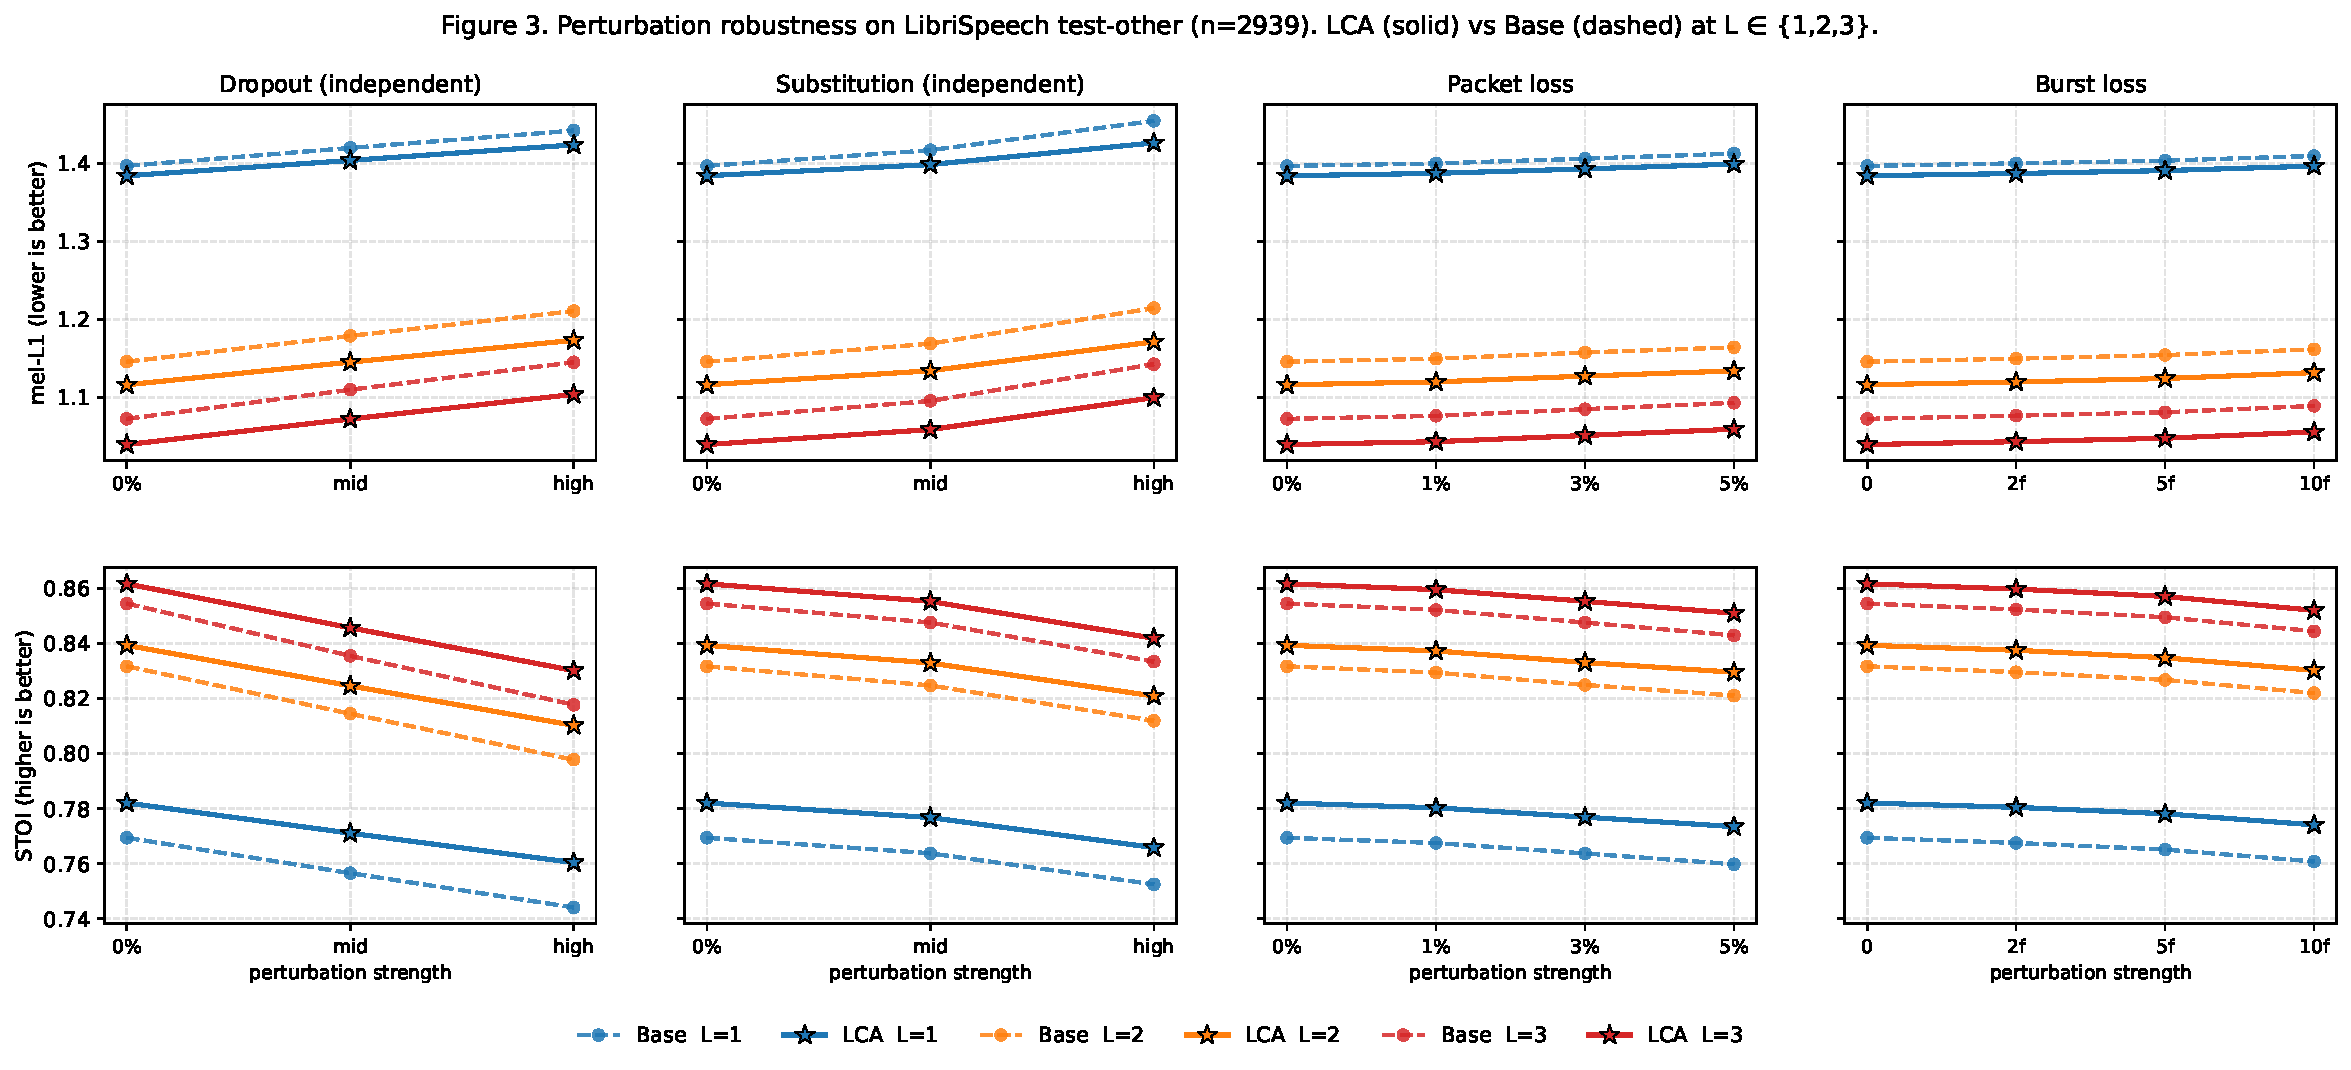
\includegraphics[width=0.95\textwidth]{figures/fig5_perturbation_robustness.pdf}
  \caption{Perturbation robustness on LibriSpeech test-other (\(n=2939\)). Solid lines are LCA, dashed lines are Base, and colors encode \(L\in\{1,2,3\}\). Across mel-L1 and STOI, LCA is consistently better under previous-frame coverage, random substitution, packet loss, and burst loss.}
  \label{fig:perturb}
\end{figure*}

Figure~\ref{fig:perturb} visualizes the test-other trend. The gap grows with perturbation strength, and the direction matches the full-set tables in the source draft.

\subsection{ASR/WER Subsets}

ASR exposes the largest practical effect of LCA. Table~\ref{tab:wer_pert} reports high-perturbation Whisper base.en results. On test-other-100, LCA lowers WER in all six cells, with reductions of 1.5--7.9 percentage points. The largest improvement is at \(L=3\) under high previous-frame coverage, from 0.485 to 0.407. On test-clean-100, LCA improves \(L=1\) but slightly hurts \(L=2,3\); per-utterance diagnostics in the source draft show that 65.0\% of the samples where LCA is worse already have Base WER below 0.1, so the degradation is concentrated near the measurement floor rather than in short utterances.

\begin{figure}[t]
  \centering
  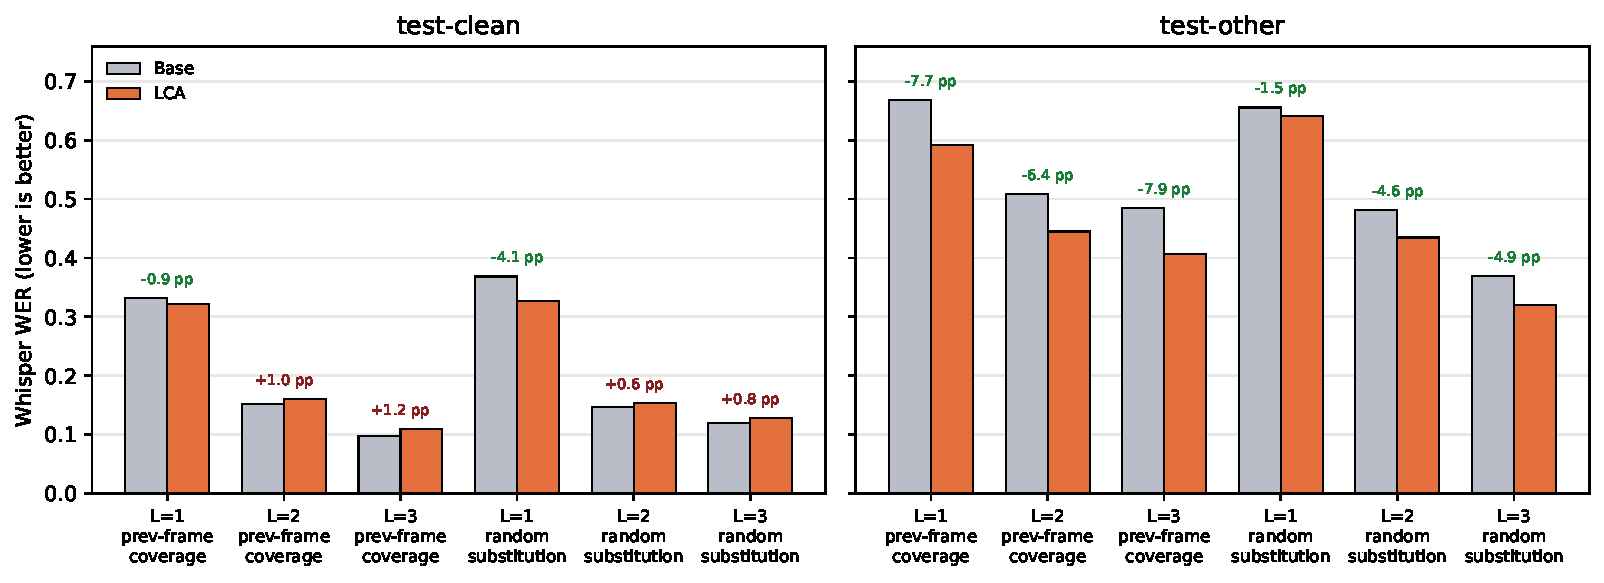
\includegraphics[width=\linewidth]{figures/fig4_perturbed_asr_wer.pdf}
  \caption{Whisper WER under high index perturbations. The annotations show LCA minus Base in percentage points. LCA consistently improves test-other, while test-clean gains are concentrated at \(L=1\).}
  \label{fig:wer}
\end{figure}

\begin{table*}[t]
\centering
\caption{Perturbed ASR results with Whisper base.en.}
\label{tab:wer_pert}
\small
\begin{tabular}{llrrrrrr}
\toprule
Subset & Condition & \(L\) & Base WER & LCA WER & \(\Delta\)WER & Base CER & LCA CER \\
\midrule
test-clean & previous-frame coverage & 1 & 0.3321 & 0.3226 & -0.0095 & 0.1801 & 0.1721 \\
test-clean & random substitution & 1 & 0.3685 & 0.3272 & -0.0413 & 0.1981 & 0.1757 \\
test-clean & previous-frame coverage & 2 & 0.1514 & 0.1610 & +0.0096 & 0.0704 & 0.0783 \\
test-clean & random substitution & 2 & 0.1464 & 0.1528 & +0.0064 & 0.0617 & 0.0792 \\
test-clean & previous-frame coverage & 3 & 0.0971 & 0.1088 & +0.0117 & 0.0398 & 0.0527 \\
test-clean & random substitution & 3 & 0.1199 & 0.1278 & +0.0079 & 0.0494 & 0.0529 \\
\midrule
test-other & previous-frame coverage & 1 & 0.6690 & 0.5921 & -0.0769 & 0.4466 & 0.3799 \\
test-other & random substitution & 1 & 0.6556 & 0.6409 & -0.0147 & 0.4179 & 0.4165 \\
test-other & previous-frame coverage & 2 & 0.5088 & 0.4449 & -0.0639 & 0.3212 & 0.2596 \\
test-other & random substitution & 2 & 0.4810 & 0.4348 & -0.0462 & 0.2976 & 0.2613 \\
test-other & previous-frame coverage & 3 & 0.4852 & 0.4066 & -0.0786 & 0.3113 & 0.2321 \\
test-other & random substitution & 3 & 0.3691 & 0.3205 & -0.0486 & 0.2201 & 0.1868 \\
\bottomrule
\end{tabular}
\end{table*}

The clean ASR subset provides context: on test-other-300, LCA lowers WER at all \(L\) values (0.6986 to 0.6941, 0.4791 to 0.4625, and 0.3929 to 0.3665). On test-clean-300, LCA improves \(L=1\) and \(L=3\) and is essentially tied at \(L=2\).

\begin{table}[t]
\centering
\caption{Clean ASR results with Whisper base.en.}
\label{tab:wer_clean}
\small
\resizebox{\linewidth}{!}{%
\begin{tabular}{llrrrr}
\toprule
Subset & \(L\) & Base WER & LCA WER & \(\Delta\)WER & \(\Delta\)CER \\
\midrule
test-clean & 1 & 0.3350 & 0.3089 & -0.0261 & -0.0160 \\
test-clean & 2 & 0.1304 & 0.1320 & +0.0016 & +0.0037 \\
test-clean & 3 & 0.1167 & 0.0933 & -0.0234 & -0.0178 \\
test-other & 1 & 0.6986 & 0.6941 & -0.0045 & -0.0217 \\
test-other & 2 & 0.4791 & 0.4625 & -0.0166 & -0.0095 \\
test-other & 3 & 0.3929 & 0.3665 & -0.0263 & -0.0077 \\
\bottomrule
\end{tabular}
}
\end{table}

\subsection{English Cross-corpus Zero-shot}

VCTK is used only for English cross-corpus zero-shot evaluation, with no retraining or fine-tuning. Table~\ref{tab:vctk} shows \base{} clean reconstruction on 300 VCTK samples compared with LibriSpeech test-clean full-set values. Mel-L1 rises only modestly, and PESQ-WB is higher on VCTK, while STOI drops from the LibriSpeech values. More importantly, \(L\) remains a valid communication knob on VCTK: as \(L\) increases from 1 to 3, mel-L1 decreases from 1.288 to 0.978, STOI increases from 0.759 to 0.821, and PESQ-WB increases from 1.477 to 2.106. This supports a restrained conclusion: waveform and spectral reconstruction transfer reasonably across English corpora, but intelligibility under accent and recording-condition shift remains weaker.

\begin{table}[t]
\centering
\caption{English cross-corpus zero-shot clean reconstruction for \base{}.}
\label{tab:vctk}
\small
\resizebox{\linewidth}{!}{%
\begin{tabular}{lrrrrrr}
\toprule
\(L\) & LS mel & VCTK mel & LS STOI & VCTK STOI & LS PESQ & VCTK PESQ \\
\midrule
1 & 1.226 & 1.288 & 0.801 & 0.759 & 1.308 & 1.477 \\
2 & 0.976 & 1.029 & 0.864 & 0.805 & 1.726 & 1.903 \\
3 & 0.907 & 0.978 & 0.885 & 0.821 & 1.954 & 2.106 \\
\bottomrule
\end{tabular}
}
\end{table}

\subsection{System Prototype Validation}
\label{sec:prototype}

We implement a three-user central-router TCP prototype to validate that the shared-codebook index-transmission interface can be placed in an endpoint loop. Figure~\ref{fig:router} shows the prototype architecture. The system contains one router and three clients A/B/C. Each client loads the same \lca{} checkpoint and pre-shared RVQ codebooks, packs the first \(L\) index layers using 10 bits per index, sends one stream, receives two streams, and decodes locally. The router forwards index packets by room only: it does not decode, mix, or access the codebooks. The prototype uses the same NAS encoder and interface parameters as the LCA recipe, with checkpoint SHA256 prefix `af60223b'. A packet-level XOR path is present only to demonstrate ciphertext-style forwarding and is not a security claim.

\begin{figure*}[t]
  \centering
  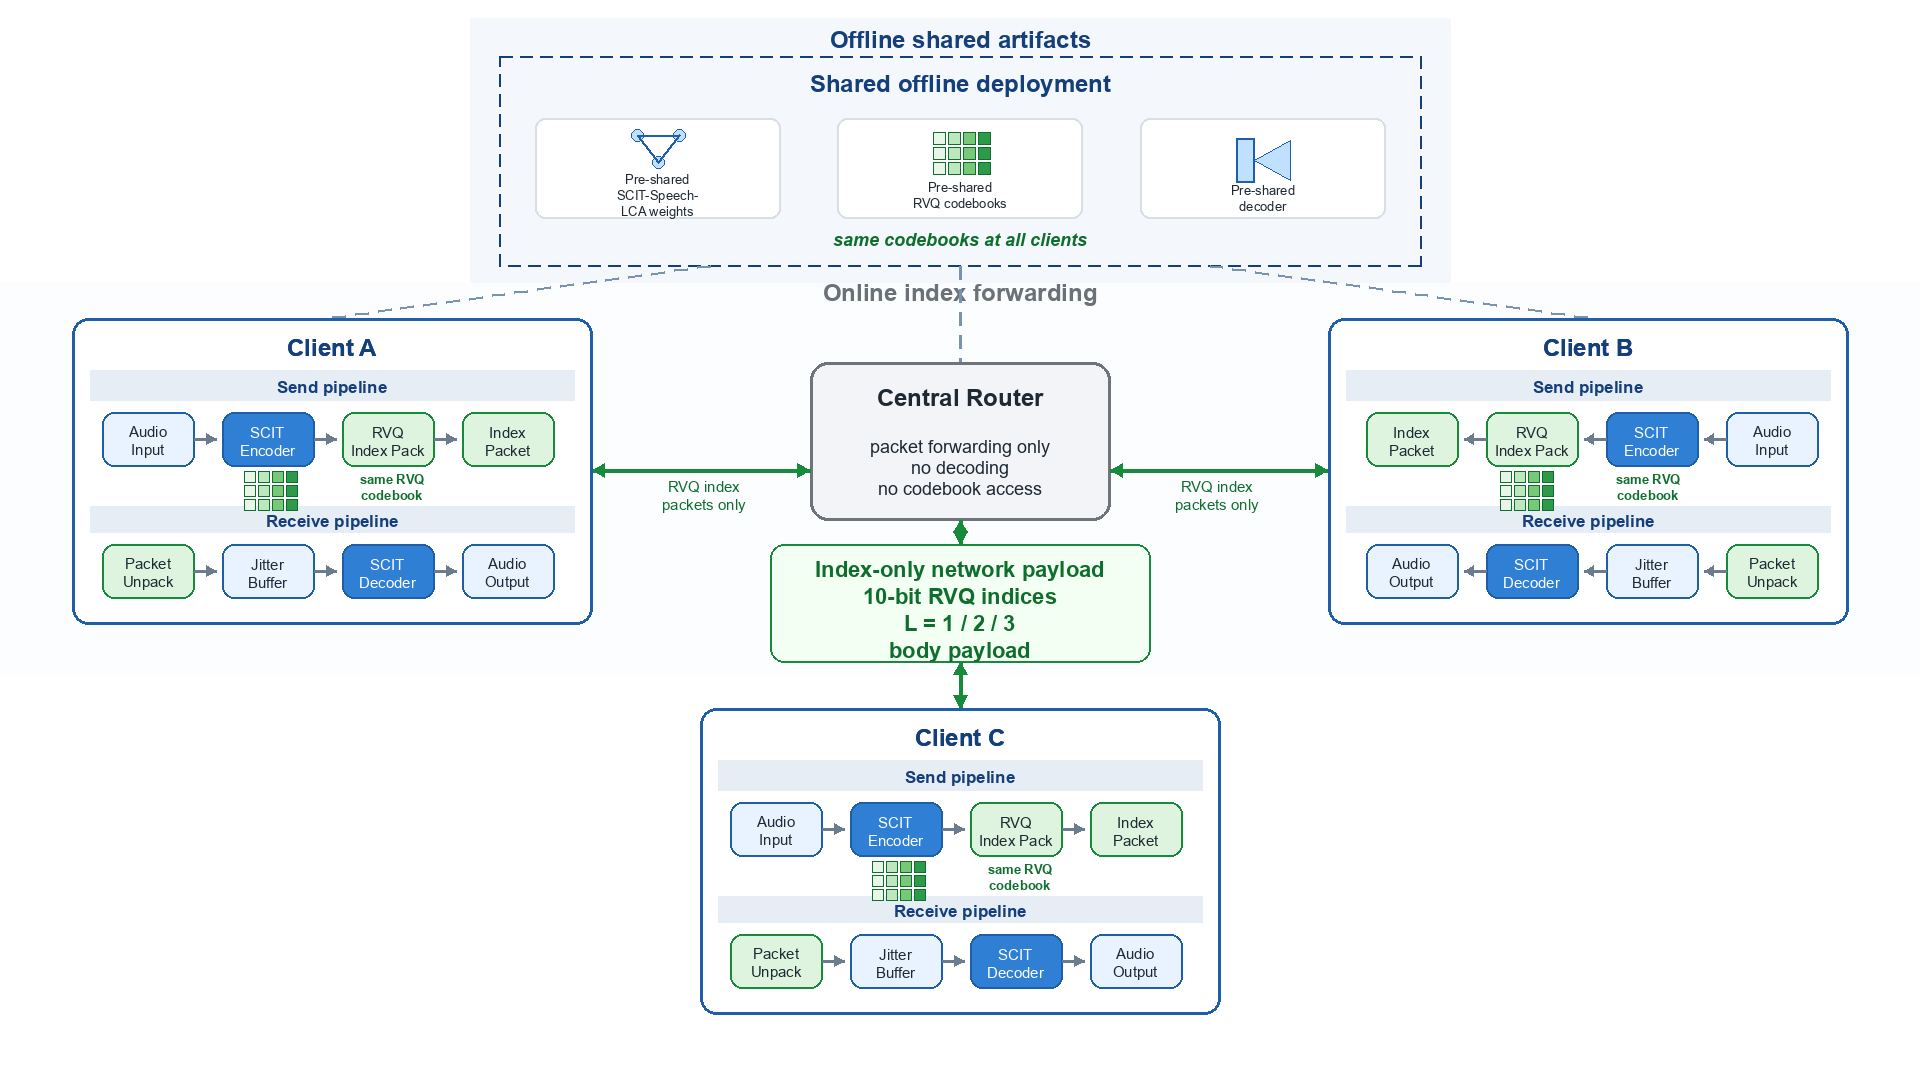
\includegraphics[width=0.95\textwidth]{figures/fig7_three_user_router_architecture.png}
  \caption{Three-user central-router prototype architecture. All clients pre-share the same \lca{} weights, RVQ codebooks, and decoder. Runtime clients send RVQ index packets to the central router; the router performs packet forwarding only and does not decode or access codebooks.}
  \label{fig:router}
\end{figure*}

Table~\ref{tab:prototype} reports single-machine TCP loopback results. A/B/C repeatedly stream the same fixed wav; each endpoint sends one stream and receives two. Each \((\mathrm{device},L)\) setting runs for 60 s on GPU and CPU. The real-time chunk is 0.5 s, corresponding to 25 latent frames, and the target jitter buffer is 0.25 s, giving an approximate one-way latency budget of 0.75 s. CPU and GPU encode/decode RTF are below 1. Per-end body bandwidth grows approximately as \(3\times 500L\) bps because each endpoint sends one stream and receives two. Per-end total bandwidth is 11.5--14.5 kbps, dominated by TCP, JSON headers, and small-packet overhead.

\begin{table}[t]
\centering
\caption{Three-client TCP prototype measurement. RTF entries are mean / worst endpoint mean.}
\label{tab:prototype}
\small
\resizebox{\linewidth}{!}{%
\begin{tabular}{lrrrrrr}
\toprule
Device & \(L\) & Single bps & Body/total kbps & Enc. RTF & Dec. RTF & Jitter/Drop \\
\midrule
GPU & 1 & 500 & 1.44 / 11.48 & 0.043 / 0.045 & 0.023 / 0.036 & 0.750 / 0 \\
GPU & 2 & 1000 & 2.85 / 12.97 & 0.041 / 0.042 & 0.022 / 0.035 & 0.750 / 0 \\
GPU & 3 & 1500 & 4.26 / 14.41 & 0.050 / 0.060 & 0.036 / 0.047 & 0.750 / 0 \\
CPU & 1 & 500 & 1.46 / 11.65 & 0.198 / 0.251 & 0.168 / 0.186 & 0.750 / 0 \\
CPU & 2 & 1000 & 2.88 / 13.03 & 0.216 / 0.225 & 0.166 / 0.186 & 0.750 / 0 \\
CPU & 3 & 1500 & 4.30 / 14.48 & 0.179 / 0.222 & 0.176 / 0.204 & 0.750 / 0 \\
\bottomrule
\end{tabular}
}
\end{table}

\section{Ablation}

This section contains one ablation theme: the factorized contribution of the three LCA components. We train V0--V3 variants and compare them with V4, the official LCA recipe. Evaluation uses a unified 256-sample train-clean-100 subset, five channel conditions, three \(L\) values, and paired random seeds for each sample, operating point, and channel condition.

\begin{table}[t]
\centering
\caption{LCA factorized variants.}
\label{tab:variants}
\small
\begin{tabular}{lccc}
\toprule
Variant & random \(L\) & ChannelSim & Consistency \\
\midrule
V0 & no & clean only & no \\
V1 & yes & clean only & no \\
V2 & no & strong & no \\
V3 & yes & strong & no \\
V4 & yes & strong & \(\lambda=0.5\) \\
\bottomrule
\end{tabular}
\end{table}

For each \((\mathrm{sample},L,\mathrm{condition})\) cell, mel robustness improvement is defined as Base degradation minus variant degradation, where degradation is perturbed mel-L1 minus clean mel-L1. Positive values mean better robustness. Table~\ref{tab:ablation} shows the 12-cell mean and paired confidence interval. V1 alone does not improve robustness. Channel perturbation simulation turns the mean positive. Random-\(L\) on top of ChannelSim further improves robustness. Consistency loss provides the final increase from +0.00494 to +0.00742.

\begin{figure}[t]
  \centering
  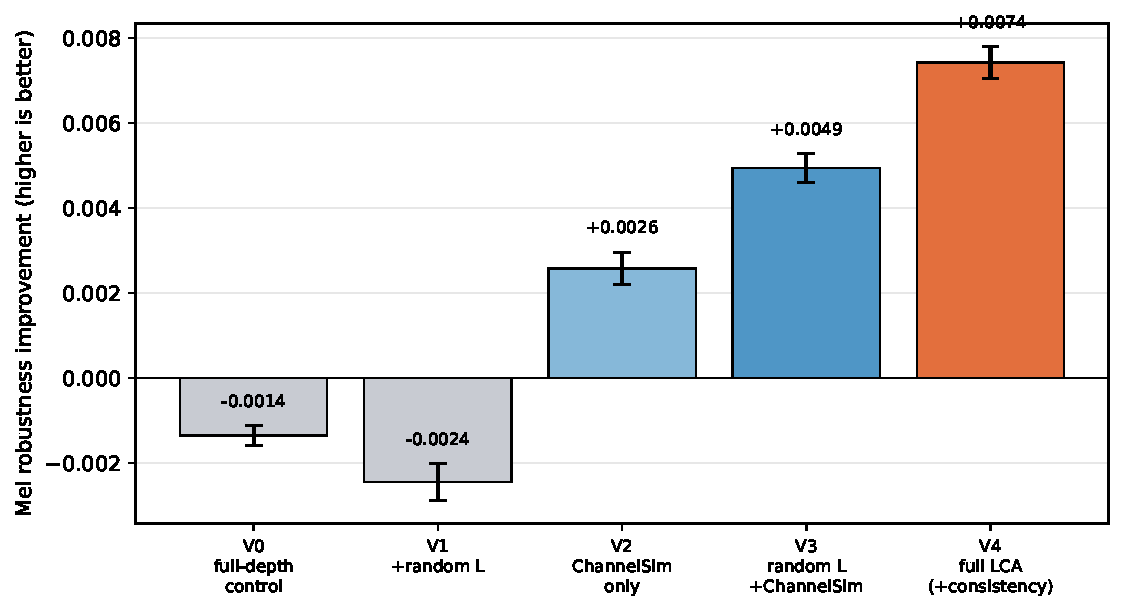
\includegraphics[width=\linewidth]{figures/fig6_lca_ablation.pdf}
  \caption{Cumulative contribution of the LCA components. Error bars are 95\% confidence intervals over the paired 256-sample, 12-cell robustness evaluation.}
  \label{fig:ablation}
\end{figure}

\begin{table}[t]
\centering
\caption{Twelve-cell mel robustness improvement for V0--V4.}
\label{tab:ablation}
\small
\begin{tabular}{lrrr}
\toprule
Variant & Mean & 95\% CI & Positive cells \\
\midrule
V0 & -0.00135 & [-0.00159, -0.00112] & 2/12 \\
V1 & -0.00245 & [-0.00288, -0.00201] & 6/12 \\
V2 & +0.00258 & [+0.00220, +0.00297] & 8/12 \\
V3 & +0.00494 & [+0.00459, +0.00527] & 12/12 \\
V4 & +0.00742 & [+0.00704, +0.00781] & 12/12 \\
\bottomrule
\end{tabular}
\end{table}

Pooled paired tests over \(12\times256=3072\) paired samples support the same reading: adding consistency loss gives V4--V3 \(=+0.00248\), \(p=7.3\times10^{-26}\); adding random \(L\) on top of ChannelSim gives V3--V2 \(=+0.00236\), \(p=1.1\times10^{-21}\); and adding ChannelSim relative to V1 gives V2--V1 \(=+0.00502\), \(p=2.5\times10^{-70}\). Although the absolute mel robustness changes are small, Section~5.5 shows that these index-level spectral stabilizations can be amplified into task-level WER reductions under difficult speech and strong perturbation.

\begin{table}[t]
\centering
\caption{Paired marginal contribution tests for LCA components.}
\label{tab:ablation_tests}
\small
\resizebox{\linewidth}{!}{%
\begin{tabular}{lrrr}
\toprule
Comparison & Pooled \(\Delta\) & \(p\)-value & Significant cells \\
\midrule
V4--V3: add consistency & +0.00248 & \(7.3\times10^{-26}\) & 10/12 \\
V3--V2: add random \(L\) over ChannelSim & +0.00236 & \(1.1\times10^{-21}\) & 4/12 \\
V2--V1: add ChannelSim over random \(L\) & +0.00502 & \(2.5\times10^{-70}\) & 12/12 \\
V4--V0: end-to-end total effect & +0.00877 & \(<10^{-256}\) & 12/12 \\
\bottomrule
\end{tabular}
}
\end{table}

The source draft further checks training dynamics by comparing the communication validation gap \( \mathrm{comm\_mel}[L,\mathrm{perturbed}]-\mathrm{comm\_mel}[L,\mathrm{clean}] \) between V4 and V3. Near the end of training, V4 has a smaller gap in 11 of 12 \((L,\mathrm{condition})\) cells, with the effect concentrated on random substitution: high random substitution shrinks by 0.067--0.101 and medium random substitution by 0.024--0.054, while previous-frame coverage changes little. This matches the mechanism: random substitution injects wrong content, and the consistency loss pulls perturbed decoding back toward the clean decoding path.

\section{Limitations}

\begin{enumerate}
  \item \textbf{Cross-corpus and real communication generalization.} We evaluate English cross-corpus zero-shot reconstruction on VCTK and validate a single-machine TCP loopback prototype. The VCTK result suggests that waveform and spectral reconstruction transfer reasonably across English speakers and accents, but STOI still drops under accent and recording-condition shift, especially at \(L=1\). The paper does not cover multilingual training, telephone or meeting speech, real devices and acoustic environments, UDP/RTP weak-network deployment, multi-machine public-network links, low-latency optimization, strict encryption, or message authentication.
  \item \textbf{Objective metrics cannot replace subjective listening.} The evidence uses mel-L1, STOI, WER, PESQ-WB, and ViSQOL, and includes AMR-WB and Codec2 comparisons. These metrics support the main same-rate neural-codec and robustness conclusions, but ViSQOL also shows that Codec2 is competitive at several low-rate points. Subjective MOS or AB tests remain necessary before claiming perceptual preference.
  \item \textbf{Codebook utilization imbalance.} Statistics over 1500 validation utterances show more than 97\% utilization in RVQ layers 2 and 3 but only about 39\% in layer 1. This is consistent with the first layer carrying frame-level semantic labels, with HuBERT distillation narrowing the semantic subspace, and with the layer-1 entropy of roughly 8 bits. Complete dead-code reinitialization fixes and utilization-quality trade-offs still require validation.
  \item \textbf{ASR subset and recognizer noise.} ASR evaluation covers 300 clean samples per LibriSpeech split and 100 perturbed samples per split, not the complete 2620/2939 utterance test sets. Whisper base.en has a nonzero PCM measurement floor, including WER about 0.075 on an eight-sample train-clean fixed diagnostic set, so WER is used mainly for relative degradation and recovery comparisons rather than as an absolute human-transcription upper bound.
\end{enumerate}

\section{Conclusion}

\method{} is a shared-codebook index-transmission speech communication system for 500--1500 bps raw/net index payloads. By pre-sharing the RVQ codebooks, model parameters, and system configuration, runtime communication reduces to transmitting the first \(L\) RVQ index layers, making \(L\) a direct operating-point knob. The NAS stage gives a lightweight transmitter encoder candidate with 86.9\% fewer parameters, 89.5\% fewer MACs, and 55.1\% lower encoder RTF than the hand-designed SEANet encoder. The Base model combines waveform, multi-scale mel, adversarial, commitment, and HuBERT distillation losses, and reaches validation mel-L1 1.12. LCA then improves low-load robustness through random operating-point sampling, strong index-level channel perturbation simulation, and mel-domain clean--perturbed consistency. Experiments show same-rate gains over DAC at 500/1000/1500 bps and over EnCodec at 1500 bps, consistent mel-L1/STOI gains under clean and perturbed full-set evaluation, task-level WER gains on difficult perturbed speech, a factorized ablation that localizes the LCA robustness source, and a restrained three-client TCP prototype demonstrating endpoint feasibility without claiming public-network, low-latency, or secure communication performance.

\bibliographystyle{IEEEtran}
\bibliography{references}

\appendix
\section*{Appendix}
\textbf{Accounting and protocol details.}

\textbf{Payload versus online bandwidth.}
The \(500L\) bps rate is the raw/net RVQ index payload under fixed 10-bit packing. It excludes packetization and protocol-stack overhead. Entropy coding could reduce the body payload to the empirical lower bounds reported in Section~3.1, while real-time protocol stacks increase online bandwidth according to packet duration and headers. The prototype's body bandwidth counts packed RVQ index payloads observed in endpoint traffic, while total bandwidth includes TCP framing, JSON headers, and payload bytes.

\textbf{ASR decoding.}
Whisper base.en uses deterministic greedy decoding and standard text normalization before WER/CER computation. The PCM passthrough lower bound is 0.0359 WER on test-clean-300 and 0.1552 WER on test-other-300.

\textbf{NAS boundary.}
The NAS search protocol is used to identify a transmitter encoder candidate under a fixed communication interface. Its short-distillation and proxy reconstruction losses are ranking proxies only. The final reconstruction and robustness claims in the paper are based on the fully trained \base{} and \lca{} checkpoints.

\textbf{Additional same-rate baselines.}

The source Chinese draft contains the full 23-method per-method tables, AMR-WB and Codec2 sweeps, and paired Wilcoxon tables. The English main text carries the key operating points needed for the 500--1500 bps claim. Codec2 700C has an actual packed bitrate around 815 bps, Codec2 1200 is around 1.2 kbps, Codec2 1300 is around 1.4 kbps, and AMR-WB 6.6 kbps has an actual packed bitrate around 7.2 kbps. SI-SNR for Codec2 and AMR-WB is not interpreted as a quality metric because codec delay and frame alignment can dominate sample-wise waveform alignment.


\end{document}

